% 3. Парадигмы программирования. Отражение в архитектуре вычислительных систем

\chapter{Парадигмы программирования. Отражение в архитектуре вычислительных систем}

\section{Определение парадигмы программирования}

Во многом особенности систем программирования определяются архитектурой исполнителей, разнообразие которых порождает множество подходов к решению даже одной и той же задачи. Это позволяет использовать различные комбинации специализированных моделей и ведет к появлению разных стилей программирования, определяемых также как парадигмы.

Парадигмы занимают важное место в технологии разработки программного обеспечения. Вокруг них начинают выстраиваться и развиваться методологические концепции. Такая роль обуславливается тем, что возникающие новые идеи по созданию программ первоначально реализуются в простых инструментах, поддерживающих исследование и экспериментальную проверку выдвигаемого стиля. Чаще всего в качестве инструментов выступают языки программирования. Упомянутые исследования начинаются с написания простых программ. Лишь после обобщения первоначального опыта приходит понимание достоинств и недостатков, позволяющих перейти к формированию методологий, обеспечивающих использование парадигмы при разработке больших программных систем. Если разработанная парадигма не способна служить основой промышленной методологии, она отвергается или применяется в ограниченных масштабах.

Существуют разнообразные определения парадигм программирования. По этому вопросу трудно найти консенсус. Поэтому каждому приходится выбирать, на чьей стороне быть. Не знаю, какая из них темная, а какая светлая, но мне ближе определение, прочитанное в свое время в книгах Гради Буча~\cite{Booch92} и~\cite{Booch98}:

\textit{Парадигма программирования – это парадигма, определяющая некоторый цельный набор идей и рекомендаций, формирующих стиль и технику написания программ. Например, в объектно-ориентированном программировании программист рассматривает программу как набор взаимодействующих объектов, тогда как в функциональном программировании программа представляется в виде цепочки вычисления функций.}

В свое время оно мне показалось ближе к общему понятию парадигмы, прочитанному в англо-русско-немецко-французском толковом словаре по вычислительной технике~\cite{ERD-dict}:

% (от греческого παράδειγμα – пример, модель, образец)
\textit{Парадигма --- в философии, социологии исходная концептуальная схема, модель постановки проблем и их решения, методов исследования, господствующих в течение определенного исторического периода в научном сообществе. Смена парадигм представляет собой научную революцию или  эволюционный переход.}

Наличие разнообразных стилей написания программ во много обусловлено гибкостью программирования, когда одни и те же идеи можно выразить различным способом. Вместе с тем реальная практика показывает, что зачастую использование соответствующего стиля программирования позволяет повысить эффективность разработки ПО в той или иной предметной области за счет большего соответствия между ее понятиями и конструкциями, предоставляемыми системами программирования.

\section{Разделение систем программирования по парадигмам}

Системы программирования, включающие языки программирования, являются основным инструментом, используемым для написания, преобразования и выполнения программ программ, что определяет их значимость в достижении критериев качества. Анализ организации систем программирования позволяет выделить специфику инструментальных средств, поддерживающих разработку программных систем.

Классификация систем программирования по парадигмам является одной из наиболее популярных. Она позволяет осуществить достаточно четкую градацию, опираясь на основные отличительные признаки. Буч [Буч98], ссылаясь в своих книгах Боброва и Стетика, приводит пять основных стилей (таблица~\ref{table-par}).

\begin{table}[h]
    \caption{Основные стили программирования по Боброву и Стетику}
    \centering
    \begin{tabular}{ | l | l | }
        \hline
        \textbf{Название стиля} & \textbf{Основополагающие абстракции} \\ \hline
        Логико-ориентированный & Цели, часто выраженные в терминах \\
        & исxисления предикатов \\ \hline
        Ориентированный на правила & Правила <<если-то>> \\ \hline
        Ориентированный на ограничения & Инвариантные отношения \\ \hline
        Процедурный & Алгоритмы, абстрактные типы данных \\ \hline
        Объектно-ориентированный & Классы и объекты \\ \hline
    \end{tabular}
    \label{table-par}
\end{table}

Для некоторых из представленных вариантов можно провести дополнительную градацию. В частности, процедурно-ориентированный стиль содержит императивную и функциональную парадигмы программирования.

\textbf{Императивное программирование} базируется на основе автоматной модели вычислителя, разделяющей абстракции состояния и поведения. При этом программа рассматривается как процесс изменения состояния путем выполнения отдельных команд. Примерами таких вычислителей являются машина Тьюринга, фон-неймановская архитектура. Различные направления императивного программирования получили широкое развитие. Из него, например, выросло структурное программирование.

\textbf{Функциональное программирование} опирается на теорию рекурсивных функций. Акцент делается на зависимость между функциями по данным. Модель состояний при этом практически игнорируется. В целом программу можно написать без явного указания последовательности вычислений, которая определяется как особенностями данных, так и тем, каким образом неявное управление вычислениями преобразуется системой программирования в явное при выполнении в реальных императивных исполнителях.

Перерастание парадигмы в методологию определяется различными факторами, среди которых можно выделить:

\begin{itemize}
    \item эффективность реализации инструментальных средств, поддерживающих исследуемую парадигму;
    \item удобство в использовании на этапе проектирования;
    \item эффективная поддержка процесса разработки больших программ;
    \item генерация эффективного выходного представления;
    \item эффективное выполнение полученной программы.
\end{itemize}

Из стилей, представленных в таблице 3.1, только процедурный и объектно-ориентированный оказались в настоящее время жизнеспособными для разработки больших программных систем. И только ООП послужило основой для разработки всеобъемлющей и сквозной методологии проектирования. Такая ситуация возникла из-за ряда особенностей, присущих различным парадигмам. Большинство из них, в конечном итоге, не смогли удовлетворить требованиям, предъявляемым к промышленным системам, так как не обеспечили комплексную поддержку разнообразных критериев качества. Поэтому, использование многих стилей в настоящий момент ограничено научными исследованиями, быстрой разработкой прототипов, учебными задачами.

Приведенная классификация, как и многие другие, построена по эмпирическому принципу, предполагающему смещения акцента на одну из специфических характеристик. При разработке систем программирования достаточно часто происходит совместная реализация нескольких парадигм, то есть, используется мультипарадигменный стиль. Подобное смешение обуславливается двумя факторами.

Во-первых, различные ключевые характеристики, акцентируют внимание на несвязанных между собою параметрах. Например, объектная ориентированность, модульность и абстрактные типы характеризуют разные подходы к конструированию программных объектов и конкурируют между собой. С другой стороны существуют различные методы алгоритмизации задач (императивный, функциональный, автоматный, логический), допускающие интеграцию с различными конструктивными элементами. Поэтому возможные сочетания невзаимосвязанных характеристик позволяют создавать системы программирования, обладающие необходимой функциональной и конструктивной полнотой для решения любых задач.

Во-вторых, особенности ряда критериев, размещаемых в одной группе, с неодинаковой эффективностью обеспечивают решение различных классов задач. Существуют языки программирования, которые, несмотря на избыточность, поддерживают различные методы конструирования программных объектов и способы описания алгоритмов. Например, ОО и процедурный подход сочетаются в C++ и Delphi, функциональное и ОО программирование одновременно могут использоваться при программировании на языках Caml и Clean. Язык программирования CLOS позволяет применять функциональный, императивный и ОО стили. Одновременное присутствие нескольких парадигм обеспечивает большую гибкость при разработке программ.

\section{Дополнительные характеристики парадигм программирования}

Независимо от используемых подходов, системы программирования обеспечивают техническую поддержку процесса разработки, который характеризуется использованием ряда общих принципов, обуславливаемых целью: создание программы, допускающей дальнейшее выполнение непосредственно или после цепочки формальных и автоматических преобразований. Вместе с тем, представленная классификация систем программирования, опирающаяся на парадигмы, не позволяет объективно и всесторонне оценить параметры, определяющие различные способы написания программ. Это затрудняет:

\begin{itemize}
    \item исследование критериев качества программного обеспечения;
    \item создание моделей для оценки различных характеристик систем программирования;
    \item разработку новых методов построения программ.
\end{itemize}

При исследовании разнообразных критериев качества программ нужно опираться не только на общие черты, определяемые парадигмами. Необходимо выделить характеристики, обеспечивающие независимый анализ требуемых характеристик. В этом случае формирование общего восприятии анализируемой системы может быть достигнуто путем комбинирования альтернативных критериев. Подобное разбиение можно провести по следующим составляющим:

\begin{enumerate}
    \item методам алгоритмизации решаемой задачи (МА);
    \item методам композиции программных объектов и формированию отношений между ними (МК);
    \item методам задания однозначности (МЗО);
    \item методам управления вычислениями (МУВ);
    \item уровням абстракции (УА);
    \item способам выполнения программ (СВП);
    \item …
\end{enumerate}


Каждая из представленных характеристик оказывает определенное влияние на особенности разрабатываемых программ.


\subsection{Методы алгоритмизации}

Описание алгоритма решаемой задачи является одной из основных задач программирования. Разнообразие методов алгоритмизации порождает множество поведенческих парадигм, каждая из которых характеризуется своей спецификой описания процесса обработки данных. Например (но далеко не все):

\begin{itemize}
    \item императивный стиль определяет исполнителя на основе традиционной фон-неймановской архитектуры, непосредственно исполняющего команды, заданные программистом (при этом команды явно связаны между собой только по управлению, а зависимость по данным выстраивается на основе образных ассоциаций программиста);
    \item автоматное программирование является подмножеством императивного стиля, акцентируясь при этом на модели состояний, что ведет к абстрагированию на этапе разработки программы от операций, связанных с обработкой данных (это ускоряет построение общей схемы логического управления алгоритмом).
    \item функциональное программирование опирается на теорию рекурсивных функций и описывает процесс управления в виде отношений между функциями (управление явно не задается и определяется зависимостью между функций по готовности результатов);
    \item программирование, управляемое потоками данных, как и функциональное программирование, использует отношение между функциями и операциями, но непосредственно ориентировано на выполнение операций по готовности данных (в отличие от функционального программирование основной упор делается на продвижение потоков, которые одновременно и параллельно запускают не связанные между собой операторы);
    \item логическое программирование опирается на логику исчисления предикатов, которая обуславливает организацию алгоритма, непосредственно не описывающую вычисления (используемая для его выполнения машина логического вывода первоначально осуществляет анализ правил, задающих различные отношения, выбирая среди них на выполнение те, которые соответствуют заданным условиям).

\end{itemize}

Каждый из представленных стилей определяет специфическую интерпретацию понятий, связанных с поведением программы и обуславливает конкретные методы и приемы построения алгоритмов, которые могут сильно отличаться даже для одной и той же решаемой задачи.


\subsection{Методы композиции программных объектов}

Разработка больших программных систем изначально опиралась на различные методы композиции. В ходе исторического развития были опробованы различные схемы компоновки структур данных и кода программы. Ряд их используется и в настоящее время. Наиболее типичными примерами являются:

\begin{itemize}
    \item процедуры (подпрограммы, функции, методы);
    \item абстрактные типы данных;
    \item классы;
    \item модули;
    \item пространства имен;
    \item интерфейсы…
\end{itemize}

В отличие от методов алгоритмизации, методы композиции программных объектов не определяют процесс выполнения решаемой задачи. Однако они оказывают существенное влияние на такие характеристики, как повторное использование кода, эволюционное расширение в ходе добавления в программу новой функциональности. Организация программных объектов оказывает существенную роль на разработку больших программных систем. Именно она обуславливает основные тенденции в современном программировании, в частности, популярность дальнейшее развитие объектно-ориентированного подхода.

Говоря о композиции программных объектов, можно отметить, что речь идет о небольшом числе форм их конструирования. Это агрегаты и обобщения, связанные между собой непосредственно, косвенно или с использованием ассоциаций. Однако в настоящее время существуют разнообразные альтернативные подходы к формированию этих конструкций, каждый из которых обеспечивает эффективную поддержку тех или иных критериев качества. Наряду с традиционными формами конструирования, опирающимися на вложенность конструктивов, сейчас широко используются подходы, обеспечивающие поддержку полиморфизма в той или иной форме, что, в свою очередь повышает гибкость процесса разработки программного обеспечения.


\subsection{Методы задания однозначности}

\begin{itemize}
    \item статическая типизация (однозначность на уровне описания типов данных)
    \item динамическая типизация (однозначность на уровне вычисляемых тегов)
    \item операционная однозначность (на уровне кодов операций компьютера)
\end{itemize}


\subsection{Методы управления вычислениями}

Методы алгоритмизации решаемой задачи тесно связаны с походами к управлению вычислениями, разнообразие которых обуславливается способами описания параллельных вычислений. Управление может варьироваться от последовательного до задания максимального параллелизма. Оно может задаваться явно программистом или неявно, когда используются отношения между данными и автоматическое управление ресурсами. Все разнообразие методов управления раскрывается как через архитектуры вычислительных систем, так и языков последовательного и параллельного программирования.

Используемые стратегии управления вычислениями сильно влияют на переносимость параллельных программ, так как именно они непосредственно отражают все ограничения, присущие как реальной вычислительной системе, так и виртуальной машине, определяющей особенности исполнителя конкретного языка программирования.


\subsection{Уровни абстракции}

Любой современный язык программирования по уровням абстракции можно разбить на несколько метауровней.

\begin{itemize}
    \item Метауровень 0: непосредственное отображение.
    \item Метауровень 1: абстракция типов.
    \item Метауровень 2: метапрограммирование.
\end{itemize}

К нулевому метауровню следует отнести конструкции языка, непосредственно отображаемые на вычислительную систему. Это переменные, процедуры, функции… То есть все те понятия языка которые отображаются в памяти компьютера. Языки программирования только этого метауровня используют при построении любых программных объектов средства прямого описания и тиражирования (клонирования). Например, клонирование данных, встречалось в языке программирования PL/1. Одной из проблем данного способа описания является то, что его достаточно сложно оторвать от памяти для независимого исследования и переносимости.

На первом метауровне располагаются абстрактные понятия, каждое из которых позволяет описать некоторое подмножество понятий первого уровня и тиражировать эти описания, отображая автоматически их на память в соответствии с семантикой. К понятиям данного метауровня можно отнести абстрактные типы данных, описание функций с параметрами, классы…

На втором метауровне размещаются абстракции, манипулирующие понятиями первого метауровня. Не вдаваясь в детали и специфику можно отметить, что на данном уровне располагаются шаблоны ряда языков программирования, позволяющи параметризировать типы классы и т.д. Сюда же можно отнести выводимость типов в ряде языков функционального программирования.

Возможно есть и более высокие метауровни, но забираться выше не будем.


\subsection{Способы выполнения программ}

Определяют специфику процессов преобразования модели исполнителя, заданной системой программирования, в модель исполнителя, осуществляющего реальное выполнение программ. Современные программные системы зачастую являют многомодульными конструкциями. Существуют различные технологии трансляции, компоновки и выполнения таких программ, что также ведет появлению разнообразных стилей программирования. В частности, использование сборки множества модулей в один монолитный конструктив в ходе статической компоновки позволяет не задумываться о том, каким образом осуществлять связь между различными программными объектами. С другой стороны динамическая подгрузка модулей во время исполнения требует написания дополнительного кода, хотя и обеспечивает большую гибкость. Таких вариантов организации выполнения программы очень много и каждый из них требует учета тех или иных особенностей, влияя тем самым на стиль программирования.

\section{Классификация систем программирования по представленным характеристикам}

К шести представленным характеристикам, по всей видмости, еще можно что-то добавить. Однако даже и в этом случае на ту или иную систему програмирования можно посмотреть исходя из ее представления в виде следующего вектора:

\begin{center}
    \verb|P = (МА, МК, МЗО, МУВ, УА, СВП…)|,\\
\end{center}
где P - парадигматическая характеристика системы программирования; A - методы алгоритмизации, используемые в системе программирования (может использоваться несколько методов); D - способы конструирования программных объектов; E - способы выполнения программы.

Исходя из этого множество разнообразных систем программирования можно «разложить» по клеткам шестимерного пространства, размер которого определяется произведением мощностей каждой из характеристик:

\begin{center}
    \verb!S = |МА| × |МК| × |МЗО| × |МУВ| × |УА| × |СВП|…!
\end{center}
Это «разложение» позволяет более гибко охарактеризовать различные системы программирования как совокупность парадигм с разными характеристиками, включая и наличие нескольких парадигм одного типа.

Данная классификация позволяет характеризовать языки сразу по нескольким независимыми парметрам, образующим многомерную таблицу. Например, на рисунке~\ref{f02-01} приведены позиции ряда известных языков программирования по двум представленным характеристикам (МА+МК).

\begin{figure}[htbp]
    \centering
    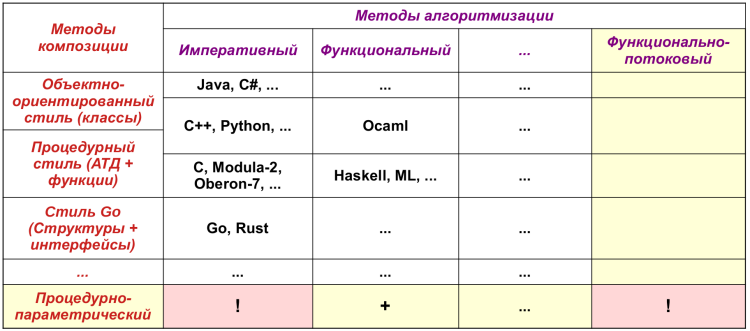
\includegraphics[width=1.0\textwidth]{img/f02-01.png}
    \caption{Классификация языков по методам алгоритмизации и методам композиции}
    \label{f02-01}
\end{figure}

